\documentclass[a4paper,12pt]{report}
\usepackage[utf8]{inputenc}
\usepackage[francais]{babel}
\usepackage{fancyhdr}
\usepackage{graphicx}
\usepackage{listings}
\usepackage{titlesec}
\usepackage{verbatim}
\usepackage{listings}
\usepackage{textcomp}
\usepackage{hyperref}
\usepackage{ amssymb }
\usepackage{longtable}



\frenchbsetup{StandardLists=true}
\newcommand{\marge}{18mm}
\usepackage[left=\marge,right=\marge,top=\marge,bottom=\marge]{geometry}
\pagestyle{fancy}
\setlength{\headheight}{14pt}
\renewcommand{\headrulewidth}{1pt}
\linespread{1}
\setlength{\columnseprule}{0.2pt}
\title{TP SCI : Simulation centrée individus}
\author{NAIT ABDELAZIZ Yanis}


\begin{document}
\maketitle
\section*{Introduction}
Dans ce TP, nous allons concevoir plusieurs systèmes multi-agents :
	Le premier simule le déplacement de particules dans un espace en deux dimensions limité. Lors de la construction d'une particule, une position initiale ainsi qu'une direction de déplacement lui sont affectées aléatoirement. Une particule, se trouvant dans un espace limité , lorsqu'elle arrive à l’extrémité de son environnement inverse la direction de son déplacement.\\
	\indent Le deuxième est un modèle de la vie des requins et des poissons se déplacent dans un espace torique ou il n'y a pas de limite. Dans ce modèle, les requins se déplacent aléatoirement et mangent les poissons se trouvant dans leur voisinage et se reproduisent tous les 10 cycles. Ces requins meurent lorsqu'ils se nourrissent pas pendant plus de 3 cycles. Les poissons se déplacent aussi aléatoirement n'ont pas besoin de se nourrir pour continuer à vivre et peuvent se reproduire tous les 10 cycles. Ces derniers peuvent mourir en se faisant manger par un requin.\\
	\indent Le troisième simule un comportement de ségrégation qui consiste à placer aléatoirement des agents de deux types différents et de leur associer un seuil de satisfaction. Chaque agent est amené à se déplacer aléatoirement tant que son taux de satisfaction est inférieur au seuil de satisfaction préalablement défini. Le taux de satisfaction de chaque individu étant égal au ratio du nombre de voisins de même type par le nombre de voisins total selon le voisinage de Moore.\\
	\indent Le quatrième est une modélisation du jeu Pacman. Dans ce jeu, il y a les fantomes qui jouent le rôle de prédateur et pacman qui joue le rôle de proie. Le principal but de ce tp est d'implémenter une stratégie de chasse des prédateurs qui permet à ces derniers d'emprunter le chemin le plus court pour atteindre sa proie en prenant en compte un certain nombre d'obstacles.

\section*{Conception}
Pour modéliser les différents acteurs, nous avons utilisé la notion d'agent autonome vivant dans un environnement discrétisé sous forme de grille 2 dimensions . En effet, un agent à un instant donné se trouve seul dans une case et est repéré par ses coordonnées cartésiennes.
Ci-dessous on peut voir le diagramme de classes permettant de modéliser tous les types d'agents énoncés ci-dessus:\\
\begin{figure}[!ht]
	\center 
	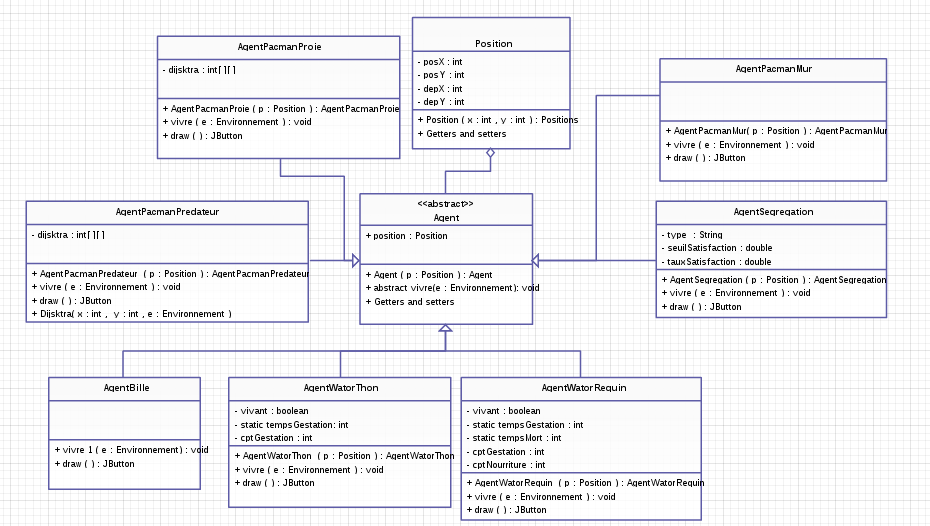
\includegraphics[scale=0.5]{./agents.png}
\end{figure}
\subsubsection*{Particules}



\begin{itemize}
\item Agent : classe mère abstraite définissant les caractéristiques communes à tous les agents. La méthode abstraite vivre sera définie dans la classe fille. L'attribut position définit la position de l'agent dans son environnement. Le comportement de chaque agent sera défini dans la méthode vivre(Environnement e).

\item Bille : classe héritant de la classe Agent. La méthode abstraite vivre décrit le comportement de la bille dans son environnement.  Une bille est animée initialement d'un mouvement aléatoire et suit toujours la même trajectoire jusqu'à atteindre la limite de son environnement ou elle inverse sa trajectoire. La collision avec une autre bille n'a pas été gérée.

\item Position : classe encapsulant des valeurs entières correspondantes aux coordonnées cartésiennes d'un agent et à la direction de déplacement de ce dernier.

\item Environnement : classe représentant l'espace dans lequel vivent les agents. Cet environnement est représenté sous forme de grille  2 dimensions. Dans chaque case de la grille peut vivre un seul agent.

\item Gui : Classe permettant d'interpréter graphiquement les données relatives aux différents agents et à l'environnement.
\end{itemize}
\noindent Ci-dessous , le rendu graphique d'une simulation du mouvement d'une bille à plusieurs instants. On remarque que lorsque la bille arrive à l'extremité de l'environnement sa direction de déplacement est inversée.
\begin{figure}[!ht]
	\center
	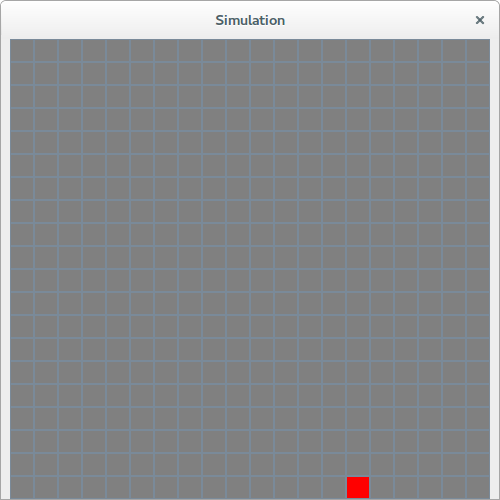
\includegraphics[scale=0.3]{./bille1.png}
	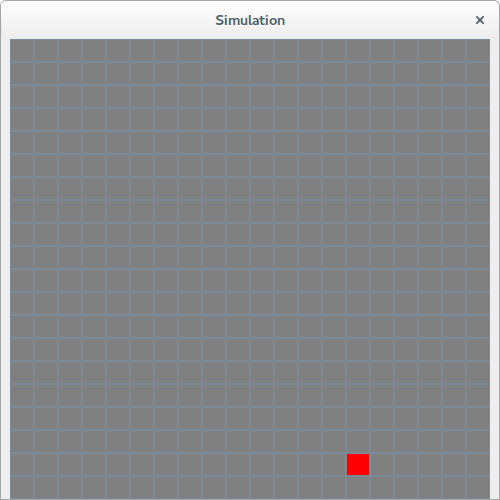
\includegraphics[scale=0.3]{./bille2.png}
\end{figure}
\noindent Pour lancer la simulation : java -jar Bille.jar width height nbBilles
\newpage
\subsubsection*{Wator}
Pour ce tp, j'ai créé deux nouvelles classes héritant de la classe Agent et une classe EnvironnementWator. La première étant la classe AgentWatorThon dont la stratégie de vie consiste à se déplacer aléatoirement dans le voisinage de Moore et à se reproduire dès que celà est possible. La deuxième étant la classe AgentWatorRequin dont la stratégie de vie consiste à se nourrir de thons et à se reproduire dès que celà est possible et à se déplacer aléatoirement. Ci-dessous on peut voir le rendu graphique d'une simulation dans laquelle un requin est représenté par un carré bleu et un thon par un carré rouge sur une grille 20$\times$20 avec 5 requins et 50 thons initiaux:
\begin{figure}[!ht]
	\center
	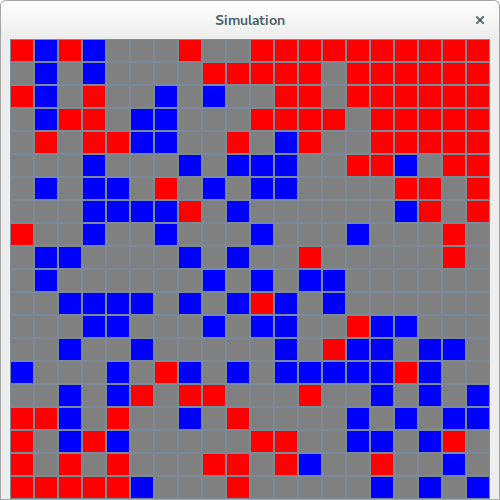
\includegraphics[scale=0.5]{./wator.png}
\end{figure} \\
\noindent Pour lancer la simulation : java -jar Wator.jar width height nbRequins nbThons 

\subsubsection*{Ségrégation}
Pour ce tp, j'ai créé une nouvelle classe AgentSegregation héritant de la classe Agent et une classe EnvironnementSegregation. Dans cette nouvelle classe d'agent, plusieurs attributs ont été ajoutés.Ces nouveaux attributs correspondent au seuil de satisfaction, au taux de satisfaction, et au type de l'agent. Pour implémenter le comportement de ségrégation, j'ai du impléménter la méthode vivre(Environnement e) qui se charge de calculer le taux de satisfaction et d'opérer à un déplacement aléatoire dans l'environnement sur une case libre si celui-ci est inférieur au seuil de satisfaction.\\
Ci-dessous on peut voir une simulation de segrégation  avec 150 agents de couleur noir et 150 agents de couleur blanche avec des seuils de satisfaction de 0.3,0.4,0.5,0.6 :
\begin{figure}[!ht]
	\center 
	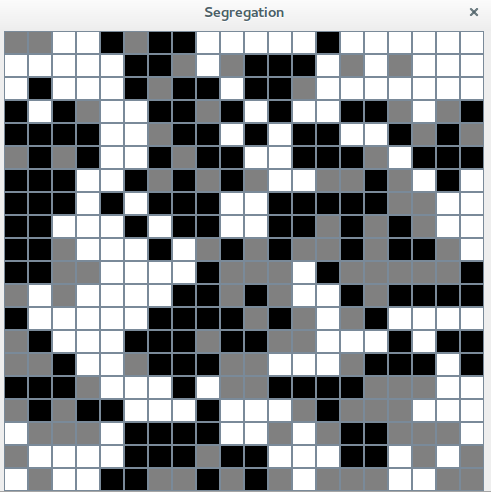
\includegraphics[scale=0.3]{150_150_30.png}
	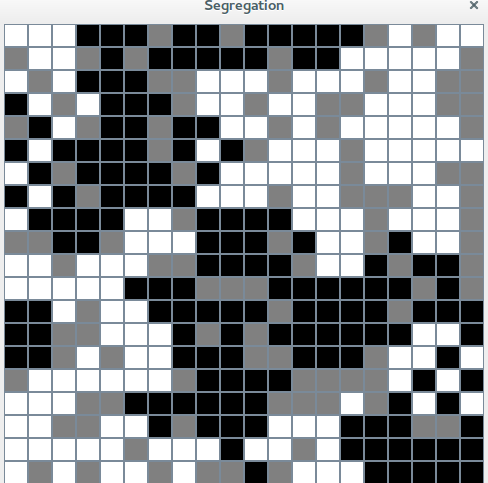
\includegraphics[scale=0.3]{150_150_40.png}
	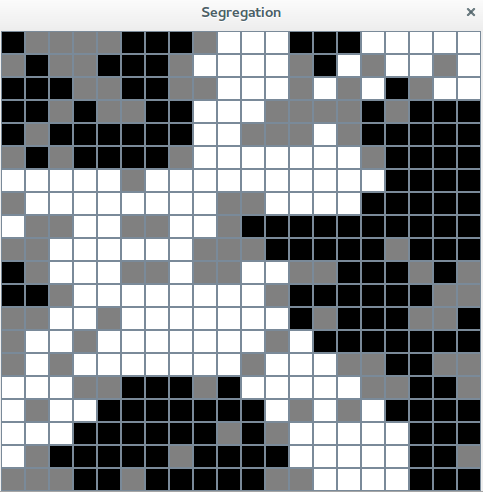
\includegraphics[scale=0.3]{150_150_50.png}
	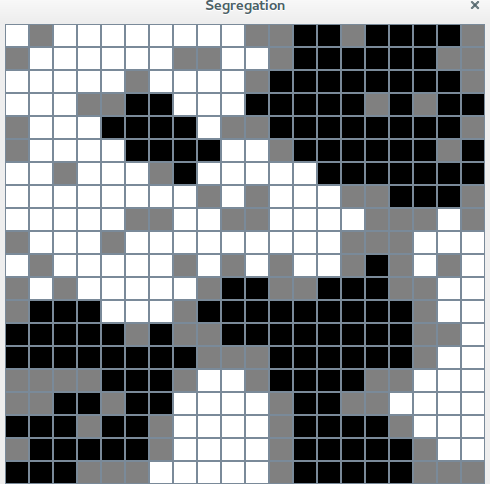
\includegraphics[scale=0.3]{150_150_60.png}
\end{figure}
\newpage
Pour les simulations ci-dessus, le calcul du taux moyen de satisfaction nous donne les résultats suivants :
\begin{center}
\begin{tabular}{|c|c|c|c|c|}
\hline
      &   seuil = 0.3 & seuil = 0.4 & seuil = 0.5 & seuil = 0.6 \\
\hline
150N/150B & 0.68 & 0.8 & 0.89 & 0.93 \\
\hline 
\end{tabular}
\end{center}
Lorsqu'on analyse les résultats ci-dessus, on remarque que le taux moyen de satisfaction est nettetment supérieur au seuil de satisfaction que nous avons fixé. Lorsque le système est stable , se forment plusieurs groupes d'entités communes.\\

\noindent Pour lancer la simulation : java -jar segregation.jar width height nbBlanc nbNoir seuilSatisfaction\\
Exemple :  java -jar segregation.jar 20 20 150 150 50
\newpage
\subsubsection*{Pacman}
Pour ce tp, j'ai créé trois nouvelles classes héritant de la classe Agent et une classe EnvironnementPacman. Tout d'abord la classe AgentPacmanMur qui représente un obstacle pour lequel la stratégie de vie consiste à rester à sa position initiale tout au long de la simulation. Puis la classe AgentPacmanProie dont la stratégie de vie consiste à se déplacer alétoirement dans une case libre dans un voisinage de 4. Et enfin la classe AgentPacmanPredateur dont la stratégie de vie consiste à se déplacer vers la proie en empruntant le plus court chemin. Pour implémenter cette stratégie de vie, nous avons utilisé l'algorithme de Dijsktra en calculant la distance minimale depuis la proie jusqu'à chaque autre de la grille. Le calcul des distances a été fait de manière récursive sur chaque case voisine de la proie. Ainsi un prédateur ayant connaissance des distances minimales de toutes les cases libres jusqu'à la proie, se déplace dans la case dans le voisinage de 4 ayant la plus petite distance. A chaque déplacement de la proie le tableau des distances est recalculé. La simulation se stabilise lorsque la proie ne peut plus fuire car elle est bloquée par le predateur. Ci-dessous on peut voir une simulation avec une proie en jaune et un prédateur en rouge positionnés aléatoirement sur une grille 10$\times$10. On voit que le prédateur suit la proie de très près.\\
\begin{figure}[!ht]
	\center
	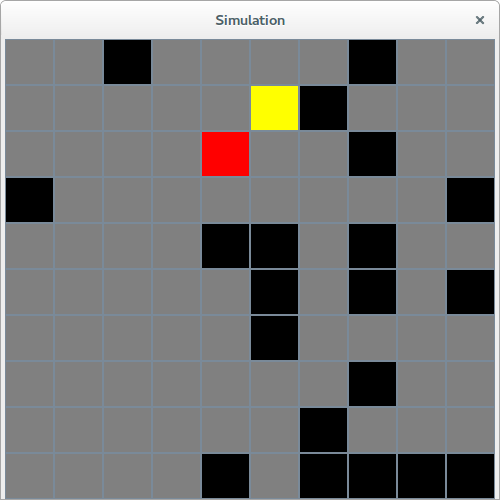
\includegraphics[scale=0.5]{./pacman.png}
\end{figure}\\
\noindent Pour lancer la simulation : java -jar Pacman.jar width height nbProies nbPredateurs
\section*{Conclusion}
A travers ces TPS, nous avons appris à apprendre le concept de programmation orientée agents en modélisant différentes simulations de comportements. On s'est rendu compte qu'à partir d'une stratégie individualiste de chaque agent, peut se dégager un comportement communautaire. 
\end{document}